\documentclass[12pt]{article}
\usepackage[utf8]{inputenc}
\usepackage[T1]{fontenc}
\usepackage[spanish]{babel}%caracteres en español
\usepackage{verbatim}
\title{\huge \textbf{\textsc{Actividad 8 \\ El sistema de Lorenz, atractores extraños y el efecto mariposa}}}%titulo en grande-negritas-versalitas
\author{Jesús Ernesto Torres Burruel}
\usepackage{graphicx}%para cargar imagenes
\graphicspath{{Imagenes/}}
\usepackage{wrapfig} %para acomodar figuras y que compartan espacio con texto
\usepackage{fancyhdr}
\pagestyle{fancy}
\fancyhf{}
\usepackage{enumerate}
\usepackage{cite}
\usepackage{hyperref}
\usepackage{bookmark}
\fancyfoot[R]{Página \thepage}
\setlength\headheight{15 pt}
\fancyhead[L]{J. Ernesto Torres Burruel}
\fancyhead[R]{Física Computacional I}
\usepackage{booktabs}
\usepackage[nottoc,numbib]{tocbibind}
\usepackage{eqnarray,amsmath}
\date{19 de mayo del 2017}
\begin{document}

\begin{titlepage}

    \begin{figure}[ht!]
    \centering
    \includegraphics[scale = 0.25]{logo}
    
    \textbf{UNIVERSIDAD DE SONORA \\ DIVISIÓN DE CIENCIAS EXACTAS Y NATURALES \\ DEPARTAMENTO DE FÍSICA \\ LICENCIATURA EN FÍSICA}
	\maketitle
    \hrule \bigskip
    \large{Física Computacional I}\\
	Profr. Carlos Lizárraga Celaya
    \end{figure}
\thispagestyle{empty}

\end{titlepage}

\newpage

\begin{center}
\huge{\textbf{\textsc{Teoría del caos y mapeo logístico}}}
\end{center}
\nocite{boeing}
\noindent La teoría del caos es un un conjunto de matématicas dedicadas al estudio de los sistemas dinámicos que son sensibles a las condiciones iniciales. El comportamiento caótico presenta características a pesar del comportamiento aleatorio que presentan los sistemas caóticos, como ciertos patrones, similitudes entre ellos, una cierta auto-organización, fractales y ciertos circuitos de retroalimentación.

El comportamiento caótico existe en muchos sistemas naturales como el clima y el estado del tiempo de la atmósfera.Existen también en las poblaciones, se tienen modelos que estiman el comportamiento de la población por su tasa de crecimiento y la población inicial, resultando en caos bajo ciertos valores para el parámetro de crecimiento. 

Existen métodos para analizar el comportamiento caótico, como el modelo matemático caótico o bien mediante técnicas analíticas como los gráficos de recurrencias o gráficos de Poincare.

La teoría del caos tiene aplicaciones en muchas disciplinas como la meteorología, la biología, sociología, física, ciencia ambiental, ciencias de la computación, economía, ingeniería y filosofía.\cite{caos}

\section{Mapeo logístico}
\noindent El mapeo logístico consiste en un modelo que busca encontrar el comportamiento de la población a partir de las condiciones en las que se encuentra, este modelo está definido con una apariencia simple, sin embargo presenta un comportamiento caótico para ciertos parámetros y valores iniciales de las poblaciones que estudia.

El modelo surgió con el fin de ubicar la situación de una población en el transcurso del tiempo considerando el crecimiento y mortalidad de la población en un solo parámetro. Este modelo solo considera a la mortalidad de la población sin considerar la influencia de otras poblaciones para que esta crezca o decrezca. 

Este es un modelo lineal de orden 2, basado en la función logística, que usa una ecuación diferencial para pasos discretos. 
El mapeo logístico se llama así porque a partir del valor de la población en cualquier tiempo cualquier tiempo encuentra el valor de la población al siguiente paso de tiempo;
matemáticamente el mapeo logístico se expresa como:
\begin{equation}
x_{t+1}=r x_t \left( 1-x_t \right)
\label{maplog}
\end{equation}
donde $x_t$ representa a la población que se estudia en cualquier tiempo t, y r es un número entero positivo que representa a razón con la que esa población crece.\cite{logmap}

\subsection{Análisis caótico del mapeo logístico}
\noindent EL mapeo logístico resulta un ejemplo bastante sencillo de analizar para mostrar los resultados que se obtienen de sistemas caóticos, ya que esta función parece bastante sencilla, pero para ciertos parámetros y valores iniciales presenta resultados caóticos.

Comencemos evaluando la función \ref{maplog} para veinte pasos de tiempo y siete distintos valores del parámetro r, $r=0.5, 1.0, ... , 3.5$.

\begin{table}[ht!]
\centering
\resizebox{0.6 \textwidth}{!}{%
\begin{tabular}{|l|l|l|l|l|l|l|l|}
\hline
 & \textbf{0.5} & \textbf{1.0} & \textbf{1.5} & \textbf{2.0} & \textbf{2.5} & \textbf{3.0} & \textbf{3.5} \\ \hline
\textbf{0} & 0.500 & 0.500 & 0.500 & 0.500 & 0.500 & 0.500 & 0.500 \\ \hline
\textbf{1} & 0.125 & 0.250 & 0.375 & 0.500 & 0.625 & 0.750 & 0.875 \\ \hline
\textbf{2} & 0.055 & 0.188 & 0.352 & 0.500 & 0.586 & 0.562 & 0.383 \\ \hline
\textbf{3} & 0.026 & 0.152 & 0.342 & 0.500 & 0.607 & 0.738 & 0.827 \\ \hline
\textbf{4} & 0.013 & 0.129 & 0.338 & 0.500 & 0.597 & 0.580 & 0.501 \\ \hline
\textbf{5} & 0.006 & 0.112 & 0.335 & 0.500 & 0.602 & 0.731 & 0.875 \\ \hline
\textbf{6} & 0.003 & 0.100 & 0.334 & 0.500 & 0.599 & 0.590 & 0.383 \\ \hline
\textbf{7} & 0.002 & 0.090 & 0.334 & 0.500 & 0.600 & 0.726 & 0.827 \\ \hline
\textbf{8} & 0.001 & 0.082 & 0.334 & 0.500 & 0.600 & 0.597 & 0.501 \\ \hline
\textbf{9} & 0.000 & 0.075 & 0.333 & 0.500 & 0.600 & 0.722 & 0.875 \\ \hline
\textbf{10} & 0.000 & 0.069 & 0.333 & 0.500 & 0.600 & 0.603 & 0.383 \\ \hline
\textbf{11} & 0.000 & 0.065 & 0.333 & 0.500 & 0.600 & 0.718 & 0.827 \\ \hline
\textbf{12} & 0.000 & 0.060 & 0.333 & 0.500 & 0.600 & 0.607 & 0.501 \\ \hline
\textbf{13} & 0.000 & 0.057 & 0.333 & 0.500 & 0.600 & 0.716 & 0.875 \\ \hline
\textbf{14} & 0.000 & 0.054 & 0.333 & 0.500 & 0.600 & 0.610 & 0.383 \\ \hline
\textbf{15} & 0.000 & 0.051 & 0.333 & 0.500 & 0.600 & 0.713 & 0.827 \\ \hline
\textbf{16} & 0.000 & 0.048 & 0.333 & 0.500 & 0.600 & 0.613 & 0.501 \\ \hline
\textbf{17} & 0.000 & 0.046 & 0.333 & 0.500 & 0.600 & 0.711 & 0.875 \\ \hline
\textbf{18} & 0.000 & 0.044 & 0.333 & 0.500 & 0.600 & 0.616 & 0.383 \\ \hline
\textbf{19} & 0.000 & 0.042 & 0.333 & 0.500 & 0.600 & 0.710 & 0.827 \\ \hline
\end{tabular}%
}
\caption{Tabla obtenida de 20 datos para 7 valores diferentes de r, las filas representan las generaciones y las columnas las tasas de crecimiento}
\label{Tabr}
\end{table}
Como se observa en la tabla \ref{Tabr} para $r= 3.5$ se observa fácilmente que tienen un comportamiento extraño.
La población para cada valor del parámetro que representa la tasa de crecimiento es siempre 0.5, eso indica cómo se comporta la población bajo distintas tasas de crecimiento.

Si analizamos la tabla al graficar las generaciones de la poblacion de acuerdo al tiempo en el que se encuentran, vemos que para algunos valores de r las poblaciones convergen en un cierto valor.

\begin{figure}[ht!]
\centering
\includegraphics[width= 0.7 \textwidth]{mapeo-logistico-tasas}
\caption{Gráfica obtenida de la tabla \ref{Tabr}, al graficar la población contra los pasos del tiempo}
\end{figure}

Existen \textit{atractores} que hacen que para algunos valores de r, la población converja a un solo valor, sin embargo a $r=3.5$ la población oscila entre varios números, este valor posee un atractor extraño, bajo el cual oscila para siempre.

\subsection{Diagramas de bifurcación }
Ahora utilicemos el mapeo logístico para 200 generaciones a través de 1,000 tasas de crecimiento entre 0.0 y 4.0. Debido a esta cantidad de datos ahora debemos obtener una visualización diferente, para ello usaremos diagramas de bifurcación. Los diagramas de bifurcación muestra los valores observados que son asintóticos para una serie de datos. \cite{bifu}

\begin{figure}[ht!]
\centering
\includegraphics[width= 0.7 \textwidth]{mapa-logistico-bifurcacion-1}
\caption{Diagrama de bifurcación obtenida al analizar 200 poblaciones para 1000 valores de r entre 0.0 y 4.0}
\label{bif1}
\end{figure}

En el diagrama de bifurcación (\ref{bif1})vemos que las poblaciones convergen a cero para las poblaciones con tasas de crecimiento menor que 1, también vemos que entre los valores de tasas de crecimiento 1 y 3 los valores convergen a un solo valor, después de $r=3.0$ vemos que oscila entre 2 valores, pero después de 3.5 comienza a oscilar entre 3 o más valores hasta llegar a oscilar en una gran cantidad de valores que se encuentran acotados.

Para observar mejor esto se hace un acercamiento al intervalo entre las tasas de crecimiento 2.8 y 4.0.

\begin{figure}[ht!]
\centering
\includegraphics[width= 0.7 \textwidth]{mapeo-logistico-bifurcacion-2}
\caption{Diagrama de bifurcación obtenido al analizar 200 poblaciones para 1000 valores de r entre 0.0 y 4.0, con acercamiento al intervalo de r entre 2.8 y 4.0}
\label{bif2}
\end{figure}

En el diagrama de bifurcación con acercamiento (figura \ref{bif2} vemos que a partir de 3 se comienza a oscilar entre dos valores, después estos se dividen en otros cuatro valores y al aumentar cada vez más los valores de r se obtienen más datos sobre los cuales oscila el mapa logístico.

Después de los valores de $r=3.5$ el mapa logistico comienza a mostrar un comportamiento caótico, pues los datos pueden oscilar entre una gran cantidad de valores. Si hacemos otro acercamiento (figura \ref{bif3}) se aprecia completamente el comportamiento caótico, pues se ven patrones, concentraciones diferentes y huecos, después de un intervalo que se presenta caos vemos que vuelve a la estabilidad donde solo toma tres valores y no una gran cantidad de ellos.

\begin{figure}[ht!]
\centering
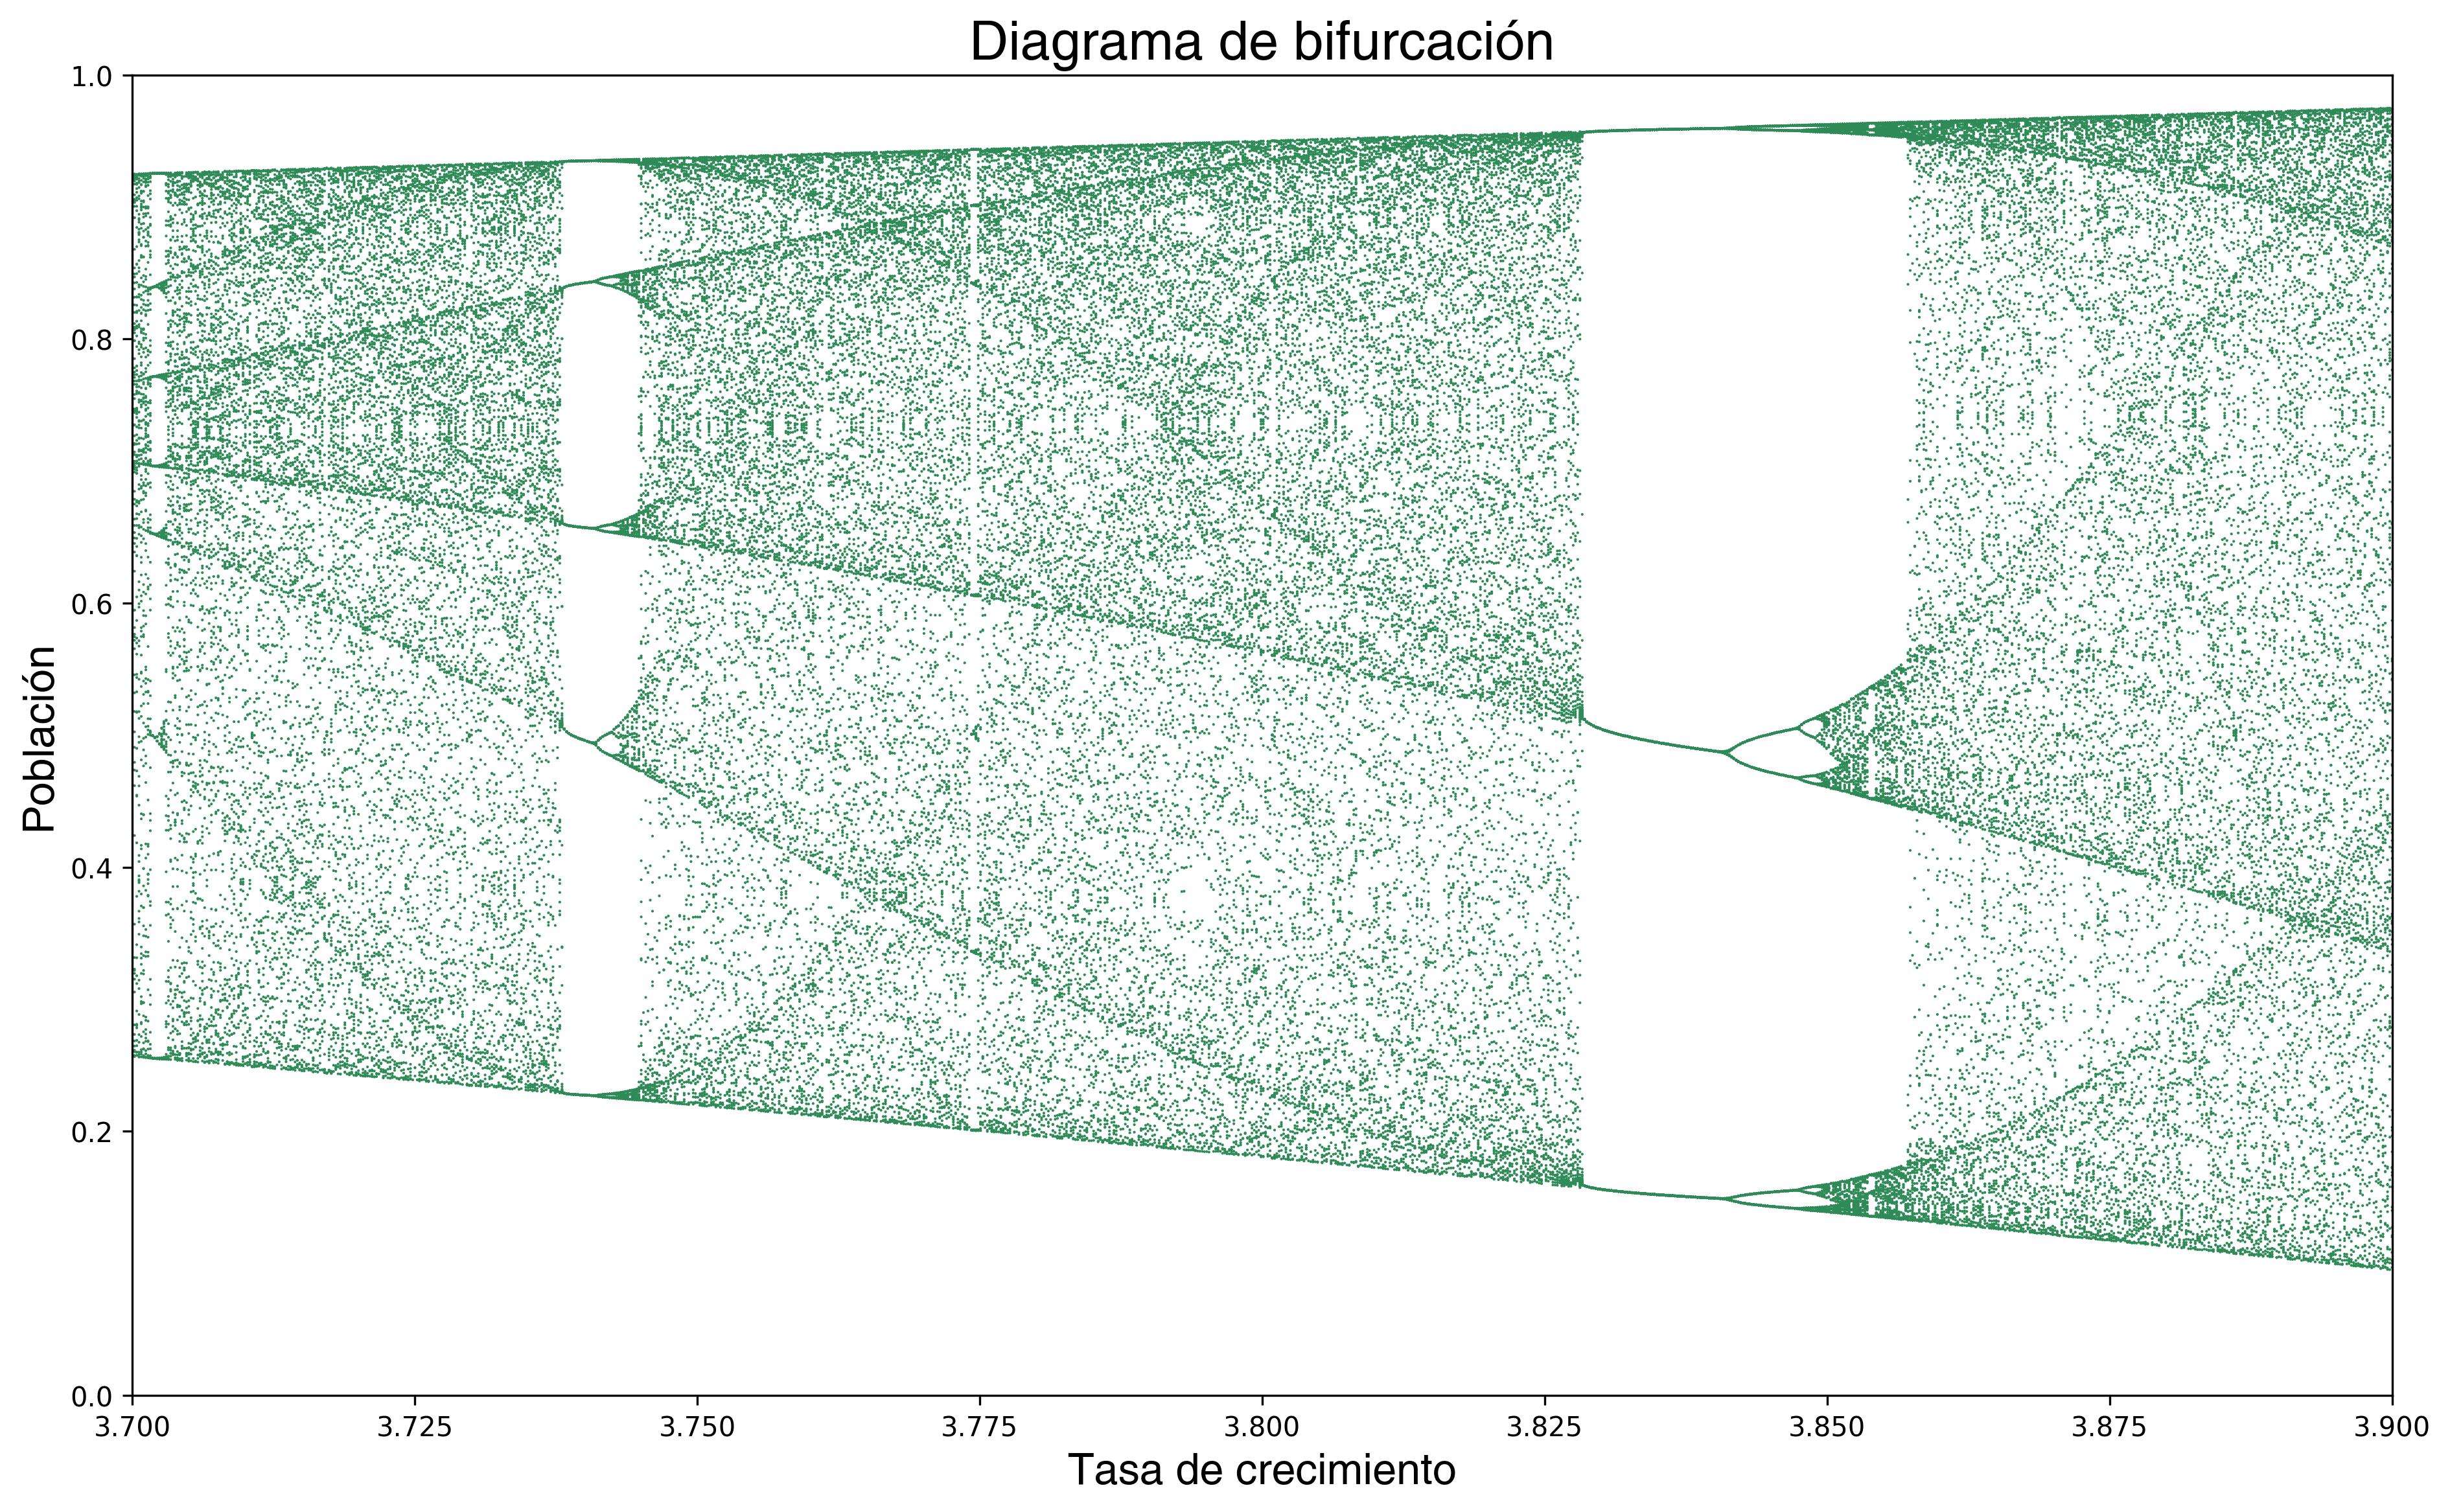
\includegraphics[width= 0.7 \textwidth]{mapeo-logistico-bifurcacion-3}
\caption{Diagrama de bifurcación obtenido al analizar 200 poblaciones para 1000 valores de r entre 0.0 y 4.0, con acercamiento al intervalo de r entre 3.7 y 3.9}
\label{bif3}
\end{figure}

\subsubsection{Fractales}
Comos e mencionó anteriormente, el comportamiento caótico presenta fractales, si realizamos un acercamiento observamos que el mapeo logístico también presenta fractales, pues en un intervalo pequeño (figura \ref{bif4} se presenta la misma bifurcación obtenida a nivel macroscópico (figura (\ref{bif1}).

\begin{figure}[ht!]
\centering
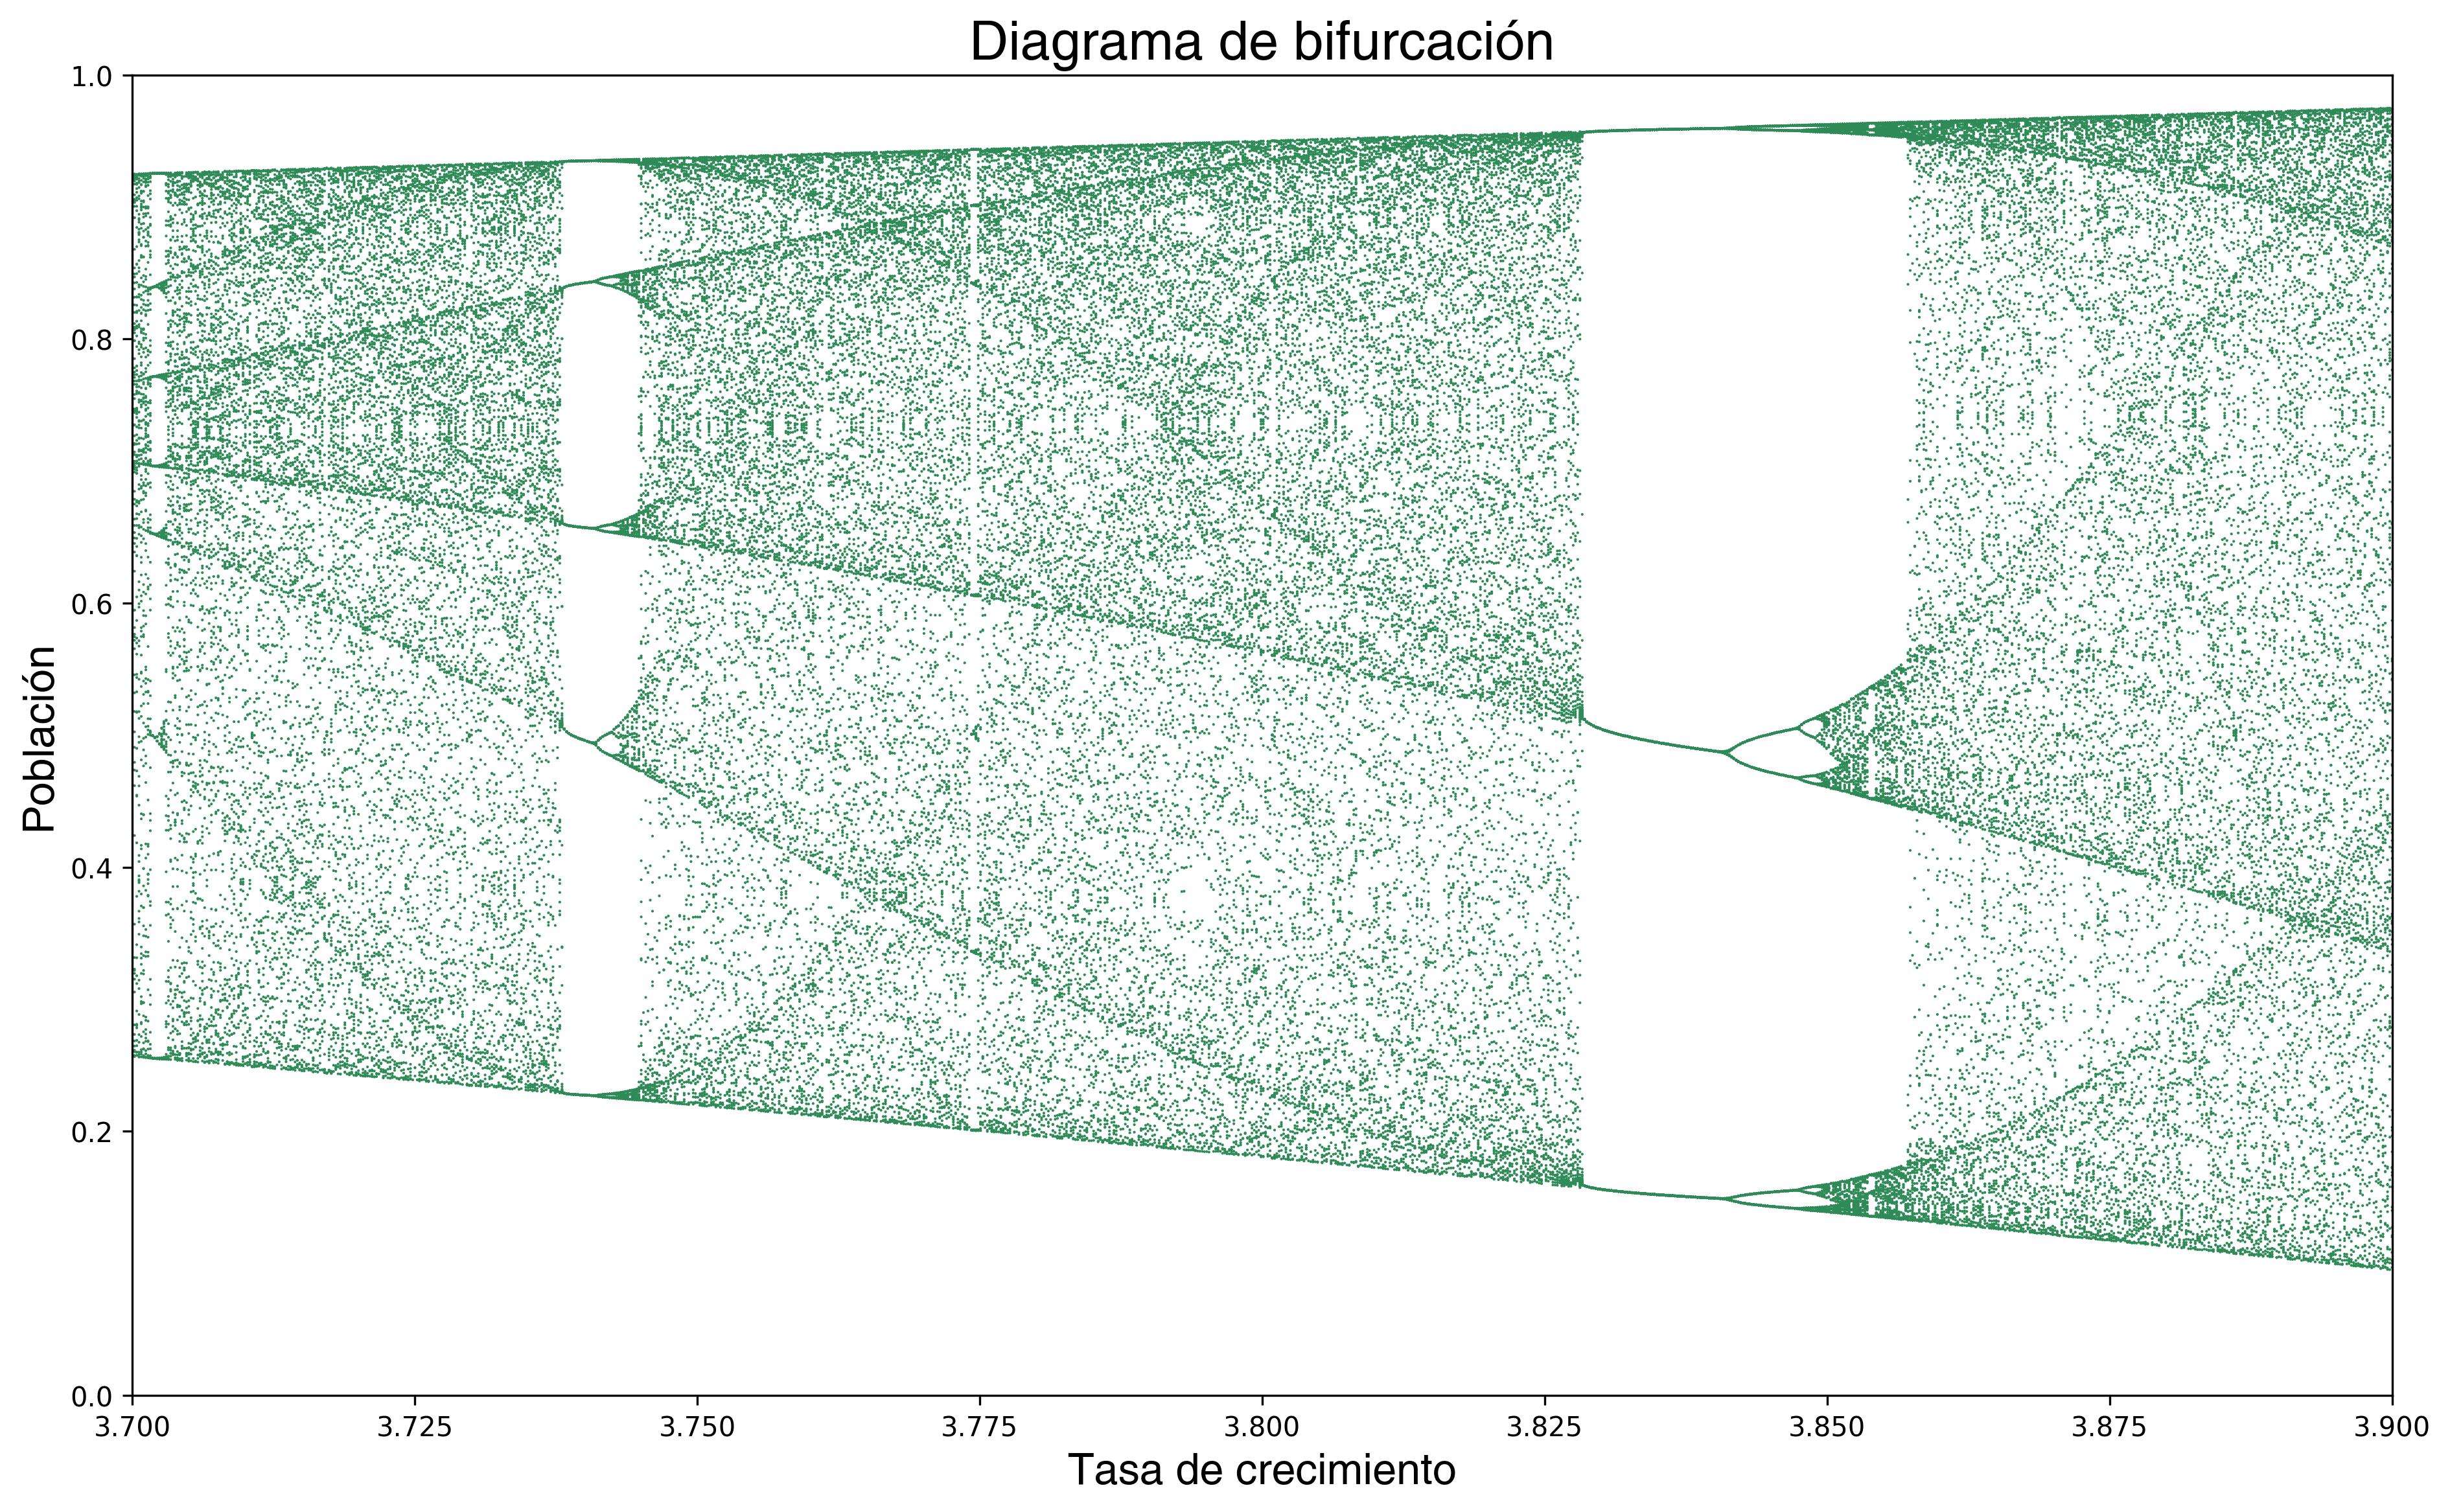
\includegraphics[width= 0.7 \textwidth]{mapeo-logistico-bifurcacion-3}
\caption{Diagrama de bifurcación obtenido al analizar 200 poblaciones para 1000 valores de r entre 0.0 y 4.0, con acercamiento al intervalo de r entre 3.840 y 3.856}
\label{bif4}
\end{figure}

\subsection{Diagramas de fase}
\noindent Otra forma de ver el comportamiento caótico es a partir de los diagramas de fase o mediante la aplicación de Poincare. Estos diagramas representan todos los posibles estados de un sistema, con cada posible estado correspondiendo a un punto único en el diagrama de fase.\cite{pcre}

Podemos hacer un análisis del mapeo logístico utilizando diagramas de fase para obtener visualizaciones del comportamiento caótico, se observa en ellos los valores que toma el mapeo logístico de acuerdo al valor de la tasa de crecimiento (figuras \ref{atr1} y \ref{atr2}).

\begin{figure}[ht!]
\centering
\includegraphics[width= 0.5 \textwidth]{atractor1}
\caption{Diagrama de fase cuando r=2.9, como se observa se encuentra un punto, que es el único valor al que converge el mapeo logístico cuando $r=2.9$, como se vio en los diagramas de bifurcación.}
\label{atr1}
\end{figure}

\begin{figure}[ht!]
\centering
\includegraphics[width= 0.5 \textwidth]{atractor2}
\caption{Diagrama de fase cuando r=3.5, como se observa se encuentran cuatro puntos, que son los cuatro valores a los que converge el mapeo logístico cuando $r=3.5$, como se vio en los diagramas de bifurcación.}
\label{atr2}
\end{figure}
\pagebreak

Para los valores en los que r presentaba un comportamiento caótico podemos ver que el diagrama de fase presenta una curva casi completa (figura \ref{atr3}).

\begin{figure}[ht!]
\centering
\includegraphics[width= 0.5 \textwidth]{atractor3}
\caption{Diagrama de fase cuando r=3.9, como se observa se encuentran una gran cantidad de puntos, que son todos los valoresque toma el mapeo logístico cuando $r=3.9$, como se vio en los diagramas de bifurcación.}
\label{atr3}
\end{figure}
\pagebreak

Si graficamos el diagrama de fase para distintos valores de r podemos obtener una serie de figuras como \ref{atr3}, solo que cada valor de la tasa de crecimiento tiene su propia curva que delimita los puntos a los que llega.

\begin{figure}[ht!]
\centering
\includegraphics[width= 0.5 \textwidth]{atractor4}
\caption{Diagrama de fase desde $r=3.6$ a $r=3.9$, como se observa se encuentran una gran cantidad de puntos, que son todos los valores que toma el mapeo logístico de acuerdo a los valores de r, como se vio en los diagramas de bifurcación.}
\label{atr4}
\end{figure}

Las figuras \ref{atr3} y \ref{atr4} muestran atractores extraños, pues los datos se encuentran sobre una misma figura, es decir, se muestra que el sistema está confinado a este patrón y oscila de manera que nunca vuelve a tomar un mismo valor.

\pagebreak
\newpage

\section{El caos contra lo aleatorio}
\noindent Es facil pensar que el caos se parece a un comportamiento aleatorio de un sistema, sin embargo hay diferencias entre el comportamiento aleatorio y el caos.

Generando una serie de datos a partir del mapeo logístico, que es un caos determinista y datos aleatorios podemos comparar su comportamiento a través de una serie de tiempo y observar las diferencias entre el caos y lo aleatorio.

\begin{figure}[ht!]
\centering
\includegraphics[width= 0.8 \textwidth]{caos-vs-aleatorio-I}
\caption{Gráfica obtenida al comparar datos caóticos contra datos aleatorios a través de una serie de tiempo}
\label{cva1}
\end{figure}
\pagebreak 
\newpage
Como vemos hay discrepancias en la serie de tiempo, sin embargo esto no ayuda bastante a identificarlos entre sí, para ello es mejor realizar diagramas de fase (de Poincare), como las figuras \ref{cva2} y \ref{cva3}

\begin{figure}[ht!]
\centering
\includegraphics[width= 0.4 \textwidth]{atractor-logistico-caos-aleatorio}
\caption{Gráfica obtenida al comparar datos caóticos contra datos aleatorios mediante un diagrama de fase}
\label{cva2}
\end{figure}

\begin{figure}[ht!]
\centering
\includegraphics[width= 0.6 \textwidth]{atractor-logistico-caos-aleatorio-3d}
\caption{Gráfica obtenida al comparar datos caóticos contra datos aleatorios mediante un diagrama de fase}
\label{cva3}
\end{figure}

Como vemos, los datos caóticos están confinados debido a atractores extraños, los datos aleatorios están dispersados sin ningún orden ni bajo ninguna restricción.

El régimen caótico del mapeo logístico se puede observar en tres dimensiones, como en la figura \ref{cva3}, podemos obtener una visualización como la figura \ref{atr4} del comportamiento caótico en 3 dimensiones, comos se ve en la figura \ref{atr5}.\footnote{ La animación de \ref{atr5} se encuentra disponible en \url{https://github.com/ErnestoTb/Computacional1/blob/master/Actividad\%209/images/fase-animada/05-diagrama-fase-logistico-3d-regimen-caotico.gif}}

\begin{figure}[ht!]
\centering
\includegraphics[width= 0.5 \textwidth]{img026}
\caption{Gráfica en 3D obtenida del diagrama de fase del mapeo logístico para valores de r entre $r=3.6$ a $r=4.0$}
\label{atr5}
\end{figure}
\pagebreak
\newpage

\section{El efecto mariposa}
\noindent El efecto mariposa surge como un término para describir que un sistema es sensible al más mínimo cambio en condiciones iniciales, como sucede con el atractor de Lorenz. En este caso el mapeo logístico también es susceptible a pequeños cambios en condiciones iniciales.

En la figura \ref{mps} vemos que dos sistemas inician de condiciones muy similares, sin embargo, después de un tiempo el comportamiento de estos sistemas difiere en gran medida, esto es una de las características de los sistemas caóticos.

\begin{figure}[ht!]
\centering
\includegraphics[width= 0.8 \textwidth]{mapa-logistico-condicion-inicial}
\caption{Gráfica obtenida de mapeo logístico al iniciar con una muy pequeña diferencia en las condiciones iniciales bajo un mismo valor de la tasa de crecimiento r}
\label{mps}
\end{figure}

\section*{Apéndice A: códigos para realizar imágenes con pynamical}
Para realizar las imágenes se utilizaron como base los códigos de ejemplo de pynamical. Debían hacerse cambios en los códigos para cambiar nombres, tamaños, colores, para ello consulté el código fuente para ver cuáles eran los argumentos clave (\*kwargs) dentro de cada comando, sobre todo en las gráficas, en general se cumplía que los títulos se cambiaban al poner como argumento "\textsf{title = 'nombre de titulo'}", de igual forma para el nombre de los ejes se usó "\textsf{xlabel}", "\textsf{ylabel}" y "\textsf{zlabel}", para los ejes $x$, $y$ y $z$, respectivamente.

Para cambiar colores de los gráficos se usaron los argumentos "\textsf{color}", "\textsf{colors}" y "\textsf{colormap}", con "color" se seleccionaba un color mediante su nombre o bien el código rgb; con "colors" y "colormap" se seleccionaba un mapa de colores de los cuales el comando iba a seleccionar una serie de colores del mapa de colores (que son paletas de colores), cada mapa de colores tiene su propio nombre. Los nombres de los colores en matplotlib pueden ser consultados en \url{https://matplotlib.org/examples/color/named_colors.html} y los nombres de los mapas de colores predeterminados se pueden consultar en \url{https://matplotlib.org/users/colormaps.html}.

Para cambiar la visualización de las figuras tridimensionales se utilizan los argumentos "\textsf{elev}" "\textsf{azim}" y "\textsf{dist}", que son las posiciones en coordenadas polares, todas están en grados; "elev" cambia la posición con respecto al eje z comenzando en la parte superior de este eje,"azim" cambia la posición con respecto a los lados (corresponde al ángulo azimutal), y "dist" cambia el alejamiento de la figura con respecto a los límites de los ejes (los límites se cambian con "\textsf{xmin}" o "\textsf{xmax}", y para los otros ejes solo se sustituye la letra inicial del argumento por "y" o "z").

Para cambiar el tamaño de cada figura se utiliza el argumento "\textsf{figsize = ("ancho", "alto")}", esto ayuda a mejorar la calidad de la imagen resultante.

A continuación se encuentran los códigos en python para elaborar las figuras, es necesario tener el paquete \textsf{pynamical} instalado.

\begin{verbatim}
# ## Mapeo logístico
# Autor: Geoff Boeing
# Artículo (Journal): Boeing, G. 2016. "Visual Analysis of Nonlinear Dynamical 
# Systems: Chaos, Fractals, Self-Similarity and the Limits of Prediction." 
# Systems, 4 (4), 37. doi:10.3390/systems4040037.
# Blog de publicación: http://geoffboeing.com/2015/03/chaos-theory-logistic-map/
# 
# *Realización de un mapa logístico y gráficas como resultados, diaramas de 
# bifurcación y diagramas de fase.
# 
# > Código editado por J. Ernesto Tb.

# In[]:

import pynamical
from pynamical import simulate, bifurcation_plot, save_fig
import pandas as pd, numpy as np, IPython.display as display, 
	matplotlib.pyplot as plt, matplotlib.cm as cm
get_ipython().magic('matplotlib inline')


# In[ ]:

title_font = pynamical.get_title_font()
label_font = pynamical.get_label_font()


# In[ ]:

# run the logistic model for 20 generations for 7 growth rates 
# between 0.5 and 3.5 
# then view the output
pops = simulate(num_gens=20, rate_min=0.5, rate_max=3.5, num_rates=7)
pops.applymap(lambda x: '{:03.3f}'.format(x))


# In[ ]:

def get_colors(cmap, n, start=0., stop=1., alpha=1., reverse=False):
    '''return n-length list of rgba colors from the passed colormap name and alpha,
       limit extent by start/stop values and reverse list order if flag is true'''
    colors = [cm.get_cmap(cmap)(x) for x in np.linspace(start, stop, n)]
    colors = [(r, g, b, alpha) for r, g, b, _ in colors]
    return list(reversed(colors)) if reverse else colors


# In[ ]:

# Grafica de los resultados del mapeo logistico para las 7 diferentes tasas de 
#crecimiento
color_list = get_colors('winter', n=len(pops.columns), start=0., stop=1)
for color, rate in reversed(list(zip(color_list, pops.columns))):
	ax = pops[rate].plot(kind='line', figsize=[15, 9], linewidth=2.5, alpha=0.95,
    c=color)
ax.grid(True)
ax.set_ylim([0, 1])
ax.legend(title='Tasa de crecimiento', loc=3, bbox_to_anchor=(1, 0.525))
ax.set_title('Resultados del modelo logístico por tasa de crecimiento', 
	fontproperties=title_font)
ax.set_xlabel('Generación', fontproperties=label_font)
ax.set_ylabel('Población', fontproperties=label_font)

save_fig('mapeo-logistico-tasas')
plt.show()


# # Bifurcación y el camino al caos

# In[ ]:

#Gráfica del diagrama de bifurcación para 200 generaciones, 
# se arrojan las primeras 100 filas
pops = simulate(num_gens=100, rate_min=0, rate_max=4, num_rates=1000, 
	num_discard=100)
bifurcation_plot(pops, title= 'Diagrama de bifurcación', 
	xlabel="Tasa de crecimiento", ylabel="Población",
	color= "palegreen", filename='mapa-logistico-bifurcacion-1',
    figsize=(15,9),
    xmin= 0., xmax=4., ymin= 0., ymax=1.2)


# In[ ]:

# corre el modelo por 200 generaciones a través de 1,000 pasos de tasas de 
# crecimiento de 2.8 a 4
# y grafica el diagrama de bifurcacion
# Esta grafica es un acercamiento al primer grafico y muestra el periodo doble del 
# camino al caos 
pops = simulate(num_gens=100, rate_min=2.8, rate_max=4, num_rates=1000,
	num_discard=200, initial_pop=0.1)
bifurcation_plot(pops, xmin=2.8, xmax=4, title= 'Diagrama de bifurcación',
	xlabel="Tasa de crecimiento", ylabel="Población",
    color= "mediumseagreen", figsize=(15,9), 
    filename='mapeo-ligistico-bifurcacion-2')


# # El comienzo del caos

# In[ ]:

# corre el modelo por 200 generaciones a través de 1,000 pasos de tasas de 
#crecimiento de 3.7 a 3.9 
# y grafica el diagrama de bifurcació
# Esta grafica es un acercamiento al primer c¿gráfico que muestra más detalles 
#en los regimenes caoticos
pops = simulate(num_gens=100, rate_min=3.7, rate_max=3.9, num_rates=1000,
	num_discard=100)
bifurcation_plot(pops, xmin=3.7, xmax=3.9, title= 'Diagrama de bifurcación', 
	xlabel="Tasa de crecimiento", ylabel="Población",
    filename='mapeo-logistico-bifurcacion-3', color = "seagreen", 
    figsize=(15,9))


# # Fractales y atractores extraños

# In[ ]:

# run the model for 500 generations across 1,000 growth rate steps 
# from 3.84 to 3.856, and plot the bifurcation diagram
# throw out the first 300 generations, so we end up with 200 generations
# this plot is a zoomed-in look at the first plot and shows 
# the same structure we saw at the macro-level
pops = simulate(num_gens=200, rate_min=3.84, rate_max=3.856, 
	num_rates=1000, num_discard=300)
bifurcation_plot(pops, xmin=3.84, xmax=3.856, ymin=0.445, ymax=0.552,
	filename='mapeo-logistico-bifurcacion-4',
    title= 'Diagrama de bifurcación', xlabel="Tasa de crecimiento",
    ylabel="Población", figsize = (15,9), color= "turquoise")


# > Diagramas de fase

# In[ ]:

import pynamical
from pynamical import simulate, save_fig, phase_diagram, phase_diagram_3d
import pandas as pd, numpy as np, matplotlib.pyplot as plt, 
	IPython.display as IPdisplay
get_ipython().magic('matplotlib inline')


# In[ ]:

title_font = pynamical.get_title_font()
label_font = pynamical.get_label_font()


# In[ ]:

# Realiza un diagrama de fase para 100 generaciones para el parámetro de 
# tasa de crecimiento r=3.1
# Muestra puntos convergiendo en 0.655 porque el mapa logistico tiene un punto 
# fijo atractor en 0.655 cuando r=2.9
pops = simulate(num_gens=100, rate_min=2.9, num_rates=1, num_discard=100)
phase_diagram(pops, title='Atractor de mapeo logístico, r=2.9',figsize= (10,10), 
		xlabel='Población(t)',ylabel='Población(t+1)', color= "winter", 
    size=25, filename= "atractor1")


# In[ ]:

# Realiza un diagrama de fase para 100 generaciones para el parámetro 
# de tasa de crecimiento r=4
# Muestra 4 puntos porque el mapa logístico tiene un período de 4 cuando r=3.5
pops = simulate(num_gens=100, rate_min=3.5, num_rates=1, num_discard=100)
phase_diagram(pops, title='Atractor de mapeo logístico, r=3.5',figsize= (10,10), 
	xlabel='Población(t)',ylabel='Población(t+1)', color= "winter", 
    size=25, filename= "atractor2")


# In[ ]:

# Realiza un diagrama de fase por 2,000 generaciones para la 
# tasa de crecimiento de 3.9
# la gráfica revela el atractor extraño - el mapa logístico 
# es caótico cuando r=3.9
pops = simulate(num_gens=2000, rate_min=3.9, num_rates=1)
phase_diagram(pops, xmin=0.25, xmax=0.75, ymin=0.8, ymax=1.01,  
	title='Atractor de mapeo logístico, r=3.9',figsize= (10,10),
    xlabel='Población(t)', ylabel='Población(t+1)',color= "winter",
    size=25, filename= "atractor3")


# In[ ]:

# Realiza un diagrama de fase para 2,000 generaciones a traves de 
# 50 tasas de crecimiento de 3.6 a 4.0
# Cada tasa de cremiento caotico tiene su propia parábola
pops = simulate(num_gens=2000, rate_min=3.6, rate_max=4.0, num_rates=50)
phase_diagram(pops, xmin=0.25, xmax=0.75, ymin=0.8, ymax=1.01, 
	title='Atractor de mapeo logístico, r=3.6 a 3.9',
    figsize= (10,10), xlabel='Población(t)', ylabel='Población(t+1)',
    color= "cool", size=7, filename= "atractor4")


# > Caos contra datos aleatorios

# In[ ]:

# A veces es dificil decir si una serie de tiempo es caotica o aleatoria
# Genera dos series de tiempo de 1,000 pasos, uno caotico y uno aleatorio
# genera 30,000 pasos de tiempo para las series caoticas pero solo mantiene las 
# 1,000 finales (si el sistema esta evolucionado)
total_gens = 30000
gens = 1000
np.random.seed(1)

chaos_pops = simulate(num_gens=total_gens, rate_min=3.99, num_rates=1)
chaos_pops = chaos_pops.iloc[total_gens-gens:].reset_index().drop(labels='index',
	axis=1)

random_pops = pd.DataFrame(np.random.random(gens), columns=['value'])
time_series = pd.concat([chaos_pops, random_pops], axis=1)
time_series.columns = ['Caos', 'Aleatorio']
time_series.head()


# In[ ]:

# grafica series de tiempo caóticas y aleatorias para mostrar 
# como son a veces para diferenciarlas 
ax = time_series.plot(kind='line', figsize=[15, 9], linewidth=3, alpha=0.6, 
style=['#003399','#cc0000'], colormap="winter")
ax.grid(True)
ax.set_xlim(40, 90)
ax.set_ylim(0, 1)
ax.set_title('Series de tiempo, Caos determinista vs Datos aleatorios', 
fontproperties=title_font)
ax.set_xlabel('Generación', fontproperties=label_font)
ax.set_ylabel('Población', fontproperties=label_font)
ax.legend(loc=3)

save_fig('caos-vs-aleatorio-l')
plt.show()


# In[ ]:

# Grafica los mismos dato como un diagrama de fase en 2D
pops = pd.concat([chaos_pops, random_pops], axis=1)
pops.columns = ['Caos', 'Aleatorio']
phase_diagram(pops, size=20, color="cool", ymax=1.005, legend=True, 
	figsize=(10,10), title = 'Gráfica Poincare, Caos vs Aleatorio',
    filename='atractor-logistico-caos-aleatorio',
    xlabel='Población(t)', ylabel='Población(t+1)')


# In[ ]:

# Grafica los mimsos datos pero en un diagrama de fase en 3D 
phase_diagram_3d(pops, color="cool", filename='atractor-logistico-caos-aleatorio-3d',
	title = 'Gráfico Poincare 3-D, Caos vs Aleatorio', xlabel='Población(t)',
	ylabel='Población(t+1)', zlabel='Población(t+2)', legend=True,
	legend_bbox_to_anchor=(0.94, 0.9), figsize= (10,10), elev=35, 
    azim=220, dist=12)

In[ ]:

# plot the numeric output of the logistic model at growth rate 
# 3.9 for 2 similar starting population values
# this demonstrates sensitive dependence on initial conditions, 
# as they diverge through chaos
r = 3.9
pops1 = simulate(num_gens=55, rate_min=r, rate_max=4.0, num_rates=1, 
	initial_pop=0.5)
pops2 = simulate(num_gens=55, rate_min=r, rate_max=4.0, num_rates=1,		
	initial_pop=0.50001)
pops = pd.concat([pops1, pops2], axis=1)
pops.columns = ['0.5', '0.50001']
ax = pops.plot(kind='line', figsize=[15, 9], linewidth=3, alpha=0.6,
	style=['#003399','#cc0000'], colormap="winter")
ax.grid(True)
ax.set_title('Resultados del modelo logístico por condiciones iniciales, 
	r={}'.format(r), fontproperties=title_font)
ax.set_xlabel('Generación', fontproperties=label_font)
ax.set_ylabel('Población', fontproperties=label_font)
ax.legend(title='Población inicial', loc=3)

save_fig('mapa-logistico-condicion-inicial')
plt.show()
\end{verbatim}

\section*{Apéndice B: Código para realizar animaciones}
\noindent Para la realización del código para crear la animación de la figura \ref{atr5} se utilizó también el código disponible en los ejemplos de pynamical.

Los argumentos utilizados para realizar cambios fueron similares a los utilizados para crear las imágenes. En este caso "color" se refiere a un mapa de colores, los nombres de los ejes se agregan con los argumentos cambian de igual forma: "\textsf{xlabel}", "\textsf{ylabel}" y "\textsf{zlabel}", para los ejes $x$, $y$ y $z$, respectivamente. Logré cambiar el nombre del archivo y la carpeta en la cual se guardaría la animación, sin embargo olvidé cambiar el título impreso en cada imagen. Debido a que compilar este cdigo y crear la animación consumió alrededor de 3 horas no realicé una animación con la correción del nombre, pero el código ya incluye el cambio del titulo impreso en la animación.

\begin{verbatim}
# > # animación en 3D

# In[ ]:

import pynamical
from pynamical import simulate, phase_diagram_3d
import pandas as pd, numpy as np, matplotlib.pyplot as plt,
	random, glob, os, IPython.display as IPdisplay
from PIL import Image
get_ipython().magic('matplotlib inline')


# In[ ]:

title_font = pynamical.get_title_font()
label_font = pynamical.get_label_font()


# In[ ]:

save_folder = 'images/fase-animada'


# In[ ]:

# run the model for 4,000 generations for 50 growth rate 
# parameters between 3.6 and 4.0
pops = simulate(num_gens=4000, rate_min=3.6, rate_max=4.0, 
	num_rates=50)

 
# In[ ]:

# set a filename and create the plot
gif_filename = '05-diagrama-fase-logistico-3d-regimen-caotico'
working_folder = '{}/{}'.format(save_folder, gif_filename)
if not os.path.exists(working_folder):
    os.makedirs(working_folder)
    
fig, ax = phase_diagram_3d(pops, color='cool',
	color_reverse=False, show=False, save=False,
    xlabel='Población (t)', ylabel='Población(t + 1)',
    zlabel='Población(t+2)')

# configure the initial viewing perspective
ax.elev = 25.
ax.azim = 321.
ax.dist = 11.0

# zoom in to reveal the 3-D structure of the strange attractor
for n in range(0, 100):
    if n <= 18:
        ax.azim = ax.azim-0.2 #begin by rotating very slowly
    if n >= 19 and n <= 29:
        ax.azim = ax.azim-10
        ax.dist = ax.dist-0.05
        ax.elev = ax.elev-2 #quickly whip around to the other side
    if n >= 33 and n <= 49:
        ax.azim = ax.azim+3
        ax.dist = ax.dist-0.55
        ax.elev = ax.elev+1.4 #zoom into the center
    if n >= 61 and n <= 79:
        ax.azim = ax.azim-2
        ax.elev = ax.elev-2
        ax.dist = ax.dist+0.2 #pull back and pan up
    if n >= 80:
        ax.azim = ax.azim-0.2 #end by rotating very slowly
    
    # add a figure title to each plot then save the figure to the disk
    fig.suptitle('Logistic Map, r=3.6 to r=4.0', fontsize=16, x=0.5, y=0.85)
    plt.savefig('{}/{}/img{:03d}.png'.format(save_folder, gif_filename, n),
    	bbox_inches='tight')

# don't display the static plot
plt.close()

# load all the static images into a list then save as an animated gif
gif_filepath = '{}/{}.gif'.format(save_folder, gif_filename)
images = [Image.open(image) for image in
	glob.glob('{}/*.png'.format(working_folder))]
gif = images[0]
gif.info['duration'] = 10 #milliseconds per frame
gif.info['loop'] = 0 #how many times to loop (0=infinite)
gif.save(fp=gif_filepath, format='gif', save_all=True, append_images=images[1:])
IPdisplay.Image(url=gif_filepath)
\end{verbatim}

\pagebreak
\newpage

\bibliographystyle{IEEEtran}
\bibliography{referencias}
\end{document}